% Created by tikzDevice version 0.12.6 on 2026-05-29 08:00:36
% !TEX encoding = UTF-8 Unicode
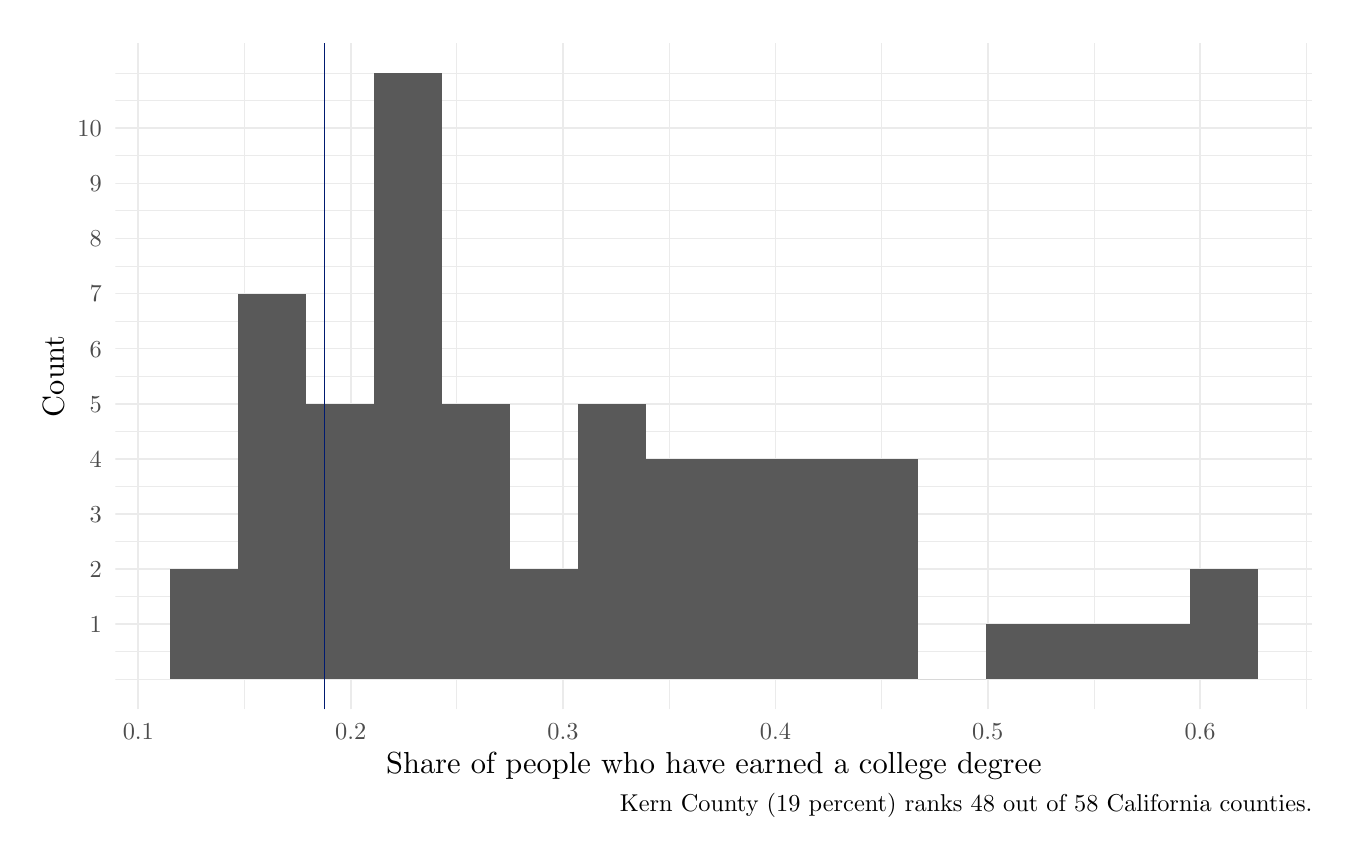
\begin{tikzpicture}[x=1pt,y=1pt]
\definecolor{fillColor}{RGB}{255,255,255}
\path[use as bounding box,fill=fillColor,fill opacity=0.00] (0,0) rectangle (469.75,290.32);
\begin{scope}
\path[clip] (  0.00,  0.00) rectangle (469.75,290.32);
\definecolor{fillColor}{RGB}{255,255,255}

\path[fill=fillColor] (  0.00,  0.00) rectangle (469.76,290.32);
\end{scope}
\begin{scope}
\path[clip] ( 31.71, 43.96) rectangle (464.25,284.82);
\definecolor{drawColor}{gray}{0.92}

\path[draw=drawColor,line width= 0.3pt,line join=round] ( 31.71, 54.91) --
	(464.25, 54.91);

\path[draw=drawColor,line width= 0.3pt,line join=round] ( 31.71, 64.86) --
	(464.25, 64.86);

\path[draw=drawColor,line width= 0.3pt,line join=round] ( 31.71, 84.77) --
	(464.25, 84.77);

\path[draw=drawColor,line width= 0.3pt,line join=round] ( 31.71,104.67) --
	(464.25,104.67);

\path[draw=drawColor,line width= 0.3pt,line join=round] ( 31.71,124.58) --
	(464.25,124.58);

\path[draw=drawColor,line width= 0.3pt,line join=round] ( 31.71,144.48) --
	(464.25,144.48);

\path[draw=drawColor,line width= 0.3pt,line join=round] ( 31.71,164.39) --
	(464.25,164.39);

\path[draw=drawColor,line width= 0.3pt,line join=round] ( 31.71,184.30) --
	(464.25,184.30);

\path[draw=drawColor,line width= 0.3pt,line join=round] ( 31.71,204.20) --
	(464.25,204.20);

\path[draw=drawColor,line width= 0.3pt,line join=round] ( 31.71,224.11) --
	(464.25,224.11);

\path[draw=drawColor,line width= 0.3pt,line join=round] ( 31.71,244.02) --
	(464.25,244.02);

\path[draw=drawColor,line width= 0.3pt,line join=round] ( 31.71,263.92) --
	(464.25,263.92);

\path[draw=drawColor,line width= 0.3pt,line join=round] ( 31.71,273.88) --
	(464.25,273.88);

\path[draw=drawColor,line width= 0.3pt,line join=round] ( 78.35, 43.96) --
	( 78.35,284.82);

\path[draw=drawColor,line width= 0.3pt,line join=round] (155.09, 43.96) --
	(155.09,284.82);

\path[draw=drawColor,line width= 0.3pt,line join=round] (231.82, 43.96) --
	(231.82,284.82);

\path[draw=drawColor,line width= 0.3pt,line join=round] (308.56, 43.96) --
	(308.56,284.82);

\path[draw=drawColor,line width= 0.3pt,line join=round] (385.29, 43.96) --
	(385.29,284.82);

\path[draw=drawColor,line width= 0.3pt,line join=round] (462.03, 43.96) --
	(462.03,284.82);

\path[draw=drawColor,line width= 0.6pt,line join=round] ( 31.71, 74.81) --
	(464.25, 74.81);

\path[draw=drawColor,line width= 0.6pt,line join=round] ( 31.71, 94.72) --
	(464.25, 94.72);

\path[draw=drawColor,line width= 0.6pt,line join=round] ( 31.71,114.62) --
	(464.25,114.62);

\path[draw=drawColor,line width= 0.6pt,line join=round] ( 31.71,134.53) --
	(464.25,134.53);

\path[draw=drawColor,line width= 0.6pt,line join=round] ( 31.71,154.44) --
	(464.25,154.44);

\path[draw=drawColor,line width= 0.6pt,line join=round] ( 31.71,174.34) --
	(464.25,174.34);

\path[draw=drawColor,line width= 0.6pt,line join=round] ( 31.71,194.25) --
	(464.25,194.25);

\path[draw=drawColor,line width= 0.6pt,line join=round] ( 31.71,214.16) --
	(464.25,214.16);

\path[draw=drawColor,line width= 0.6pt,line join=round] ( 31.71,234.06) --
	(464.25,234.06);

\path[draw=drawColor,line width= 0.6pt,line join=round] ( 31.71,253.97) --
	(464.25,253.97);

\path[draw=drawColor,line width= 0.6pt,line join=round] ( 39.98, 43.96) --
	( 39.98,284.82);

\path[draw=drawColor,line width= 0.6pt,line join=round] (116.72, 43.96) --
	(116.72,284.82);

\path[draw=drawColor,line width= 0.6pt,line join=round] (193.45, 43.96) --
	(193.45,284.82);

\path[draw=drawColor,line width= 0.6pt,line join=round] (270.19, 43.96) --
	(270.19,284.82);

\path[draw=drawColor,line width= 0.6pt,line join=round] (346.92, 43.96) --
	(346.92,284.82);

\path[draw=drawColor,line width= 0.6pt,line join=round] (423.66, 43.96) --
	(423.66,284.82);
\definecolor{fillColor}{gray}{0.35}

\path[fill=fillColor] ( 51.37, 54.91) rectangle ( 75.95, 94.72);

\path[fill=fillColor] ( 75.95, 54.91) rectangle (100.53,194.25);

\path[fill=fillColor] (100.53, 54.91) rectangle (125.10,154.44);

\path[fill=fillColor] (125.10, 54.91) rectangle (149.68,273.88);

\path[fill=fillColor] (149.68, 54.91) rectangle (174.25,154.44);

\path[fill=fillColor] (174.25, 54.91) rectangle (198.83, 94.72);

\path[fill=fillColor] (198.83, 54.91) rectangle (223.41,154.44);

\path[fill=fillColor] (223.41, 54.91) rectangle (247.98,134.53);

\path[fill=fillColor] (247.98, 54.91) rectangle (272.56,134.53);

\path[fill=fillColor] (272.56, 54.91) rectangle (297.14,134.53);

\path[fill=fillColor] (297.14, 54.91) rectangle (321.71,134.53);

\path[fill=fillColor] (321.71, 54.91) rectangle (346.29, 54.91);

\path[fill=fillColor] (346.29, 54.91) rectangle (370.87, 74.81);

\path[fill=fillColor] (370.87, 54.91) rectangle (395.44, 74.81);

\path[fill=fillColor] (395.44, 54.91) rectangle (420.02, 74.81);

\path[fill=fillColor] (420.02, 54.91) rectangle (444.59, 94.72);
\definecolor{drawColor}{RGB}{0,26,112}

\path[draw=drawColor,line width= 0.6pt,line join=round] (107.29, 43.96) -- (107.29,284.82);
\end{scope}
\begin{scope}
\path[clip] (  0.00,  0.00) rectangle (469.75,290.32);
\definecolor{drawColor}{gray}{0.30}

\node[text=drawColor,anchor=base east,inner sep=0pt, outer sep=0pt, scale=  0.88] at ( 26.76, 71.78) {1};

\node[text=drawColor,anchor=base east,inner sep=0pt, outer sep=0pt, scale=  0.88] at ( 26.76, 91.69) {2};

\node[text=drawColor,anchor=base east,inner sep=0pt, outer sep=0pt, scale=  0.88] at ( 26.76,111.59) {3};

\node[text=drawColor,anchor=base east,inner sep=0pt, outer sep=0pt, scale=  0.88] at ( 26.76,131.50) {4};

\node[text=drawColor,anchor=base east,inner sep=0pt, outer sep=0pt, scale=  0.88] at ( 26.76,151.41) {5};

\node[text=drawColor,anchor=base east,inner sep=0pt, outer sep=0pt, scale=  0.88] at ( 26.76,171.31) {6};

\node[text=drawColor,anchor=base east,inner sep=0pt, outer sep=0pt, scale=  0.88] at ( 26.76,191.22) {7};

\node[text=drawColor,anchor=base east,inner sep=0pt, outer sep=0pt, scale=  0.88] at ( 26.76,211.13) {8};

\node[text=drawColor,anchor=base east,inner sep=0pt, outer sep=0pt, scale=  0.88] at ( 26.76,231.03) {9};

\node[text=drawColor,anchor=base east,inner sep=0pt, outer sep=0pt, scale=  0.88] at ( 26.76,250.94) {10};
\end{scope}
\begin{scope}
\path[clip] (  0.00,  0.00) rectangle (469.75,290.32);
\definecolor{drawColor}{gray}{0.30}

\node[text=drawColor,anchor=base,inner sep=0pt, outer sep=0pt, scale=  0.88] at ( 39.98, 32.95) {0.1};

\node[text=drawColor,anchor=base,inner sep=0pt, outer sep=0pt, scale=  0.88] at (116.72, 32.95) {0.2};

\node[text=drawColor,anchor=base,inner sep=0pt, outer sep=0pt, scale=  0.88] at (193.45, 32.95) {0.3};

\node[text=drawColor,anchor=base,inner sep=0pt, outer sep=0pt, scale=  0.88] at (270.19, 32.95) {0.4};

\node[text=drawColor,anchor=base,inner sep=0pt, outer sep=0pt, scale=  0.88] at (346.92, 32.95) {0.5};

\node[text=drawColor,anchor=base,inner sep=0pt, outer sep=0pt, scale=  0.88] at (423.66, 32.95) {0.6};
\end{scope}
\begin{scope}
\path[clip] (  0.00,  0.00) rectangle (469.75,290.32);
\definecolor{drawColor}{RGB}{0,0,0}

\node[text=drawColor,anchor=base,inner sep=0pt, outer sep=0pt, scale=  1.10] at (247.98, 20.91) {Share of people who have earned a college degree};
\end{scope}
\begin{scope}
\path[clip] (  0.00,  0.00) rectangle (469.75,290.32);
\definecolor{drawColor}{RGB}{0,0,0}

\node[text=drawColor,rotate= 90.00,anchor=base,inner sep=0pt, outer sep=0pt, scale=  1.10] at ( 13.08,164.39) {Count};
\end{scope}
\begin{scope}
\path[clip] (  0.00,  0.00) rectangle (469.75,290.32);
\definecolor{drawColor}{RGB}{0,0,0}

\node[text=drawColor,anchor=base east,inner sep=0pt, outer sep=0pt, scale=  0.88] at (464.25,  7.21) {Kern County (19 percent) ranks 48 out of 58 California counties.};
\end{scope}
\end{tikzpicture}
